\documentclass[a4paper,12pt]{article}
% -------------------------------------------------------------------
%                  Essential packages (used in template)
% -------------------------------------------------------------------

\usepackage[utf8]{inputenc}                   % Allow Umlauts (ä, ö, ü)
\usepackage[ngerman]{babel, translator}       % German LaTeX-intern descriptors (Abbildungen, ...)
\usepackage{mathptmx}                         % Font "Times New Roman" in mathematical Environments
\usepackage{courier}                          % Support the use of font "Courier" (used in listings)
\usepackage[T1]{fontenc}                      % Change LaTeX font encoding to support modern fonts
\usepackage{fix-cm}                           % Fix sizes at which CM and EC fonts can be used

\usepackage{geometry}                         % Change text bounds on a per-page basis
\usepackage{fancyhdr}                         % Allow easy customization of headers and footers

\usepackage[ddmmyyyy]{datetime}               % Reformat times from LaTeX commands like \today

\usepackage[usenames,dvipsnames]{xcolor}      % Support text colorization

\usepackage{colortbl}                         % Support applying colors to tables
\usepackage{array}                            % Tables with fixed column size
\usepackage{longtable}                        % Support multi-page tables
\usepackage{multicol}                         % Additional settings for \multicolumn
\usepackage{multirow}                         % Additional settings for \multirow

\usepackage[hyphens,obeyspaces,spaces]{url}   % Allow urls to have line breaks at "-"
\usepackage{hyperref}                         % Clickable hyperlinks in Table of Contents
\usepackage{microtype}                        % Enable "Blocksatz"

\usepackage{float}                            % Support for table H option
\usepackage{floatflt}                         % Support text wrapping around floating environments
\usepackage{wrapfig}                          % Support text wrapping around figures

\usepackage{graphicx}                         % Support including graphics environments for images
\usepackage{caption}                          % Provide greater customization around captions
\usepackage{subcaption}                       % Caption support for subfigures

\usepackage{setspace}                         % Set line spacing to be 1.5x the default
\usepackage{listings}                         % Code block support for LaTeX

\usepackage[titles]{tocloft}                  % More options to modify list of figures & tables
\usepackage{nomencl}                          % Support for nomenclatures ("Symbolverzeichnis")

\usepackage{amsmath}                          % Includes a plethora of mathematical packages 
\usepackage{amssymb}                          % Source mathematical symbols like \sin
\usepackage{amsthm}                           % Better theorems
\usepackage{upgreek}                          % Use \Upomega to get a straight \Omega
\usepackage{siunitx}                          % Unified support for si units

\usepackage{ifthen}                           % Support better if statements in LaTeX
\usepackage{etoolbox} 						  % Easily patch commands

% Support list of acronyms and glossary
\usepackage[
	toc,
	nogroupskip,
	nonumberlist,
	nopostdot,
	acronyms,
	shortcuts,
	translate=babel
]{glossaries}

% Track the total count of different environments
% Needs to be imported because LaTeX resets these counter on a chapter basis
\usepackage[figure,table,lstlisting,xspace]{totalcount}

% Annotate different information directly into the document
\setlength{\marginparwidth}{2cm}
\usepackage[
	colorinlistoftodos,
	prependcaption,
	textsize=tiny
]{todonotes}

% -------------------------------------------------------------------
%                 Useful packages (not used in template)
% -------------------------------------------------------------------

\usepackage{pdfpages}                         % Include existing PDFs into the work

% Create electrical diagrams within LaTeX
\usepackage[
	european,
	oldvoltagedirection,
	straightvoltages,
	siunitx
]{circuitikz}
% page margins
\geometry{
	left=2.5cm,
	right=2.5cm,
	top=2.5cm,
	bottom=3cm
}

% Disable single lines at the start of a paragraph (Schusterjungen)
\clubpenalty=10000

% Disable single lines at the end of a paragraph (Hurenkinder)
\widowpenalty=10000
\displaywidowpenalty=10000

% Fixed size table columns
\newcolumntype{L}[1]{>{\raggedright\arraybackslash}p{#1}}
\newcolumntype{C}[1]{>{\centering\arraybackslash}p{#1}}
\newcolumntype{R}[1]{>{\raggedleft\arraybackslash}p{#1}}

\renewcommand{\arraystretch}{1.2}                       % Distance between lines in tables

\captionsetup{justification=raggedright}                % Align captions to the left

\setcounter{secnumdepth}{3}                             % Only allow nesting 3 layers (down to subsubsections)

% Set convention to german (comma instead of point delimiter for floats)
\sisetup{
	locale=DE,                   % Use German notation (comma instead of point delimiter for floats)
	per-mode=fraction,           % Switch display to use \frac instead of x^{-1}
	fraction-function=\tfrac,    % Use amsmath's tfrac macro for unit fractions
}

% -------------------------------------------------------------------
%                     Usability & visual changes
% -------------------------------------------------------------------

% Create a better looking header and footer
\pagestyle{fancy}
\fancyhf{}
\lhead{\nouppercase{\leftmark}}
\rfoot{\thepage}

% Automatically generate a box around figure environments
\floatstyle{boxed}
\restylefloat{figure}

% Set toc sections to be clickable
\hypersetup{
	colorlinks,
	citecolor=black,
	filecolor=black,
	linkcolor=black
}

\frenchspacing                                          % Insert one space after a sentence, not 2

\renewcommand{\UrlFont}{\color{blue}\rmfamily\itshape}  % URLs should be displayed in blue
\renewcommand{\dateseparator}{.}                        % Dates are written like 01.01.1970, not 01-01-1970

\addto{\captionsngerman}{
	\renewcommand*{\figurename}{Abb.}                     % Figures should be displayed as "Abb. x"
	\renewcommand*{\tablename}{Tab.}                      % Tables should be displayed as "Tab. x"
	\renewcommand*{\lstlistingname}{Code}                 % Code should be displayed as "Code x"
	\renewcommand*{\nomname}{Symbolverzeichnis}           % Nomenclature in German is "Symbolverzeichnis"
}

% -------------------------------------------------------------------
%                        Code listing setup
% -------------------------------------------------------------------

\lstset{
	basicstyle=\small\ttfamily\color{black}\linespread{0.5},      % Font size used for the code
	commentstyle=\ttfamily\color{gray},                           % Comment style
	keywordstyle=\ttfamily\color{blue},                           % Keyword style
	stringstyle=\color{ForestGreen!30!LimeGreen},                 % String literal style
	% frame=single,                                               % Add a frame around the code
	showstringspaces=false,                                       % Don't underline spaces within strings only
	% captionpos=b,                                               % Set caption-position to bottom
	% backgroundcolor=\color{white},                              % Background color
	tabsize=1,                                                    % Tabulatorgröße
	numbers=left,
	numberstyle=\small,
	numbersep=8pt,
	breaklines=true,
}

% To style lstlistlisting like the lof, you first have to register it
% to tocloft, as mentioned in https://tex.stackexchange.com/a/27648/27635
\makeatletter
\begingroup\let\newcounter\@gobble\let\setcounter\@gobbletwo
\globaldefs\@ne \let\c@loldepth\@ne
\newlistof{listings}{lol}{\lstlistlistingname}
\endgroup
\let\l@lstlisting\l@listings
\makeatother

% -------------------------------------------------------------------
%                         Redefining geometry
% -------------------------------------------------------------------

% Figures
\renewcommand{\cftfigpresnum}{\figurename~}
\renewcommand{\cftfigaftersnum}{:}
\setlength{\cftfignumwidth}{2cm}
\setlength{\cftfigindent}{0cm}

% Tables
\renewcommand{\cfttabpresnum}{\tablename~}
\renewcommand{\cfttabaftersnum}{:}
\setlength{\cfttabnumwidth}{2cm}
\setlength{\cfttabindent}{0cm}

% Listings
\renewcommand*{\cftlistingspresnum}{\lstlistingname~}
\renewcommand*{\cftlistingsaftersnum}{:}
\settowidth{\cftlistingsnumwidth}{\cftlistingspresnum}
\addtolength{\cftlistingsnumwidth}{1cm}
\setlength{\cftlistingsindent}{0cm}

\setlength{\parindent}{0cm}                             % Don't indent start of paragraph
\setlength{\parskip}{6pt}                               % Lines are seperated by 6pt

\setlength{\headheight}{1.25cm}
\setlength{\footskip}{1cm}
\setlength{\headsep}{1cm}

% -------------------------------------------------------------------
%                    Custom counters & commands
% -------------------------------------------------------------------

\newcounter{countacronym}
\DeclareTotalCounter{countacronym}
\newcommand*{\acr}[1]{\acrshort{#1}\stepcounter{countacronym}}
\newcommand*{\Acr}[1]{\acrlong{#1}\stepcounter{countacronym}}

\newcounter{countnomen}
\DeclareTotalCounter{countnomen}
\newcommand*{\nomen}[2]{\nomenclature{#1}{#2}\stepcounter{countnomen}}
\newcommand{\nomunit}[1]{\renewcommand{\nomentryend}{\hspace*{\fill}#1}}
\newcommand{\nomsi}[1]{\nomunit{[\si{#1}]}}

% Count number of references to the glossary
\newcounter{countglossary}
\DeclareTotalCounter{countglossary}
\pretocmd{\Gls}{\stepcounter{countglossary}}{}{}
\pretocmd{\gls}{\stepcounter{countglossary}}{}{}
\pretocmd{\Glspl}{\stepcounter{countglossary}}{}{}
\pretocmd{\glspl}{\stepcounter{countglossary}}{}{}

% TODO annotations
\newcounter{counttodo}
\DeclareTotalCounter{counttodo}
\newcommand{\note}[2][]{
	\todo[color=green!25,bordercolor=green,tickmarkheight=3pt,#1]{#2}
	\stepcounter{counttodo}
}
\newcommand{\unsure}[2][]{
	\todo[color=Plum!25,bordercolor=Plum,tickmarkheight=3pt,#1]{#2}
	\stepcounter{counttodo}
}
\newcommand{\change}[2][]{
	\todo[color=blue!25,bordercolor=blue,tickmarkheight=3pt,#1]{#2}
	\stepcounter{counttodo}
}

\newcommand{\imgref}[1]{\hyperref[#1]{Abbildung~\getrefnumber{#1}}}
\newcommand{\tabref}[1]{\hyperref[#1]{Tabelle~\getrefnumber{#1}}}
\newcommand{\coderef}[1]{\hyperref[#1]{Code~\getrefnumber{#1}}}
\newcommand{\mathref}[1]{\hyperref[#1]{Gleichung~\getrefnumber{#1}}}
\newcommand{\secref}[1]{\hyperref[#1]{Abschnitt~\getrefnumber{#1}}}

% Preload custom user settings & packages
\IfFileExists{./Custom.tex}{\newcommand{\myImageWidth}{\linewidth}
\newcommand{\myImagePos}{\centering}

\setstretch{1.2}
\usepackage{pgfplots}
\usepackage[
	backend=biber,
	style=alphabetic,
	url = false,
]{biblatex}
\DefineBibliographyStrings{ngerman}{
	andothers = {{et\,al\adddot}},
}

\usepackage{svg}

\usepackage{courier}
\usepackage{xcolor}

\colorlet{punct}{red!60!black}
\definecolor{delim}{RGB}{20,105,176}
\colorlet{numb}{magenta!60!black}

\lstdefinelanguage{json}{
literate=
*{0}{{{\color{numb}0}}}{1}
{1}{{{\color{numb}1}}}{1}
{2}{{{\color{numb}2}}}{1}
{3}{{{\color{numb}3}}}{1}
{4}{{{\color{numb}4}}}{1}
{5}{{{\color{numb}5}}}{1}
{6}{{{\color{numb}6}}}{1}
{7}{{{\color{numb}7}}}{1}
{8}{{{\color{numb}8}}}{1}
{9}{{{\color{numb}9}}}{1}
{:}{{{\color{punct}{:}}}}{1}
{,}{{{\color{punct}{,}}}}{1}
{\{}{{{\color{delim}{\{}}}}{1}
{\}}{{{\color{delim}{\}}}}}{1}
{[}{{{\color{delim}{[}}}}{1}
{]}{{{\color{delim}{]}}}}{1},
}

\usepackage{tcolorbox}
\tcbuselibrary{listings,skins}

\newtcblisting[auto counter]{mylisting}[2][]{
	arc=0pt, outer arc=0pt,
	listing only,
	title=#2,
	left=16pt,
	#1,
}}{}

\newcommand{\startHSCdocument}[1][]{

  % Register different entries: glossary, nomenclature, acronyms
  \makeglossaries
  \hyphenation{}

  % \newacronym
% [% options to override defaults
%   longplural={Forwarding Equivalence Classes},
%   shortplural={FECs}
% ]
% {fec}{FEC}{Forwarding Equivalence Class}

  \makenomenclature
  % \nomenclature[01]{\textbf{Symbol}}{\textbf{Bedeutung} \nomunit{\textbf{[phys. Einheit]}}}

  \include{Verzeichnisse/Glossar}

  % Register actual document
\begin{document}
\shorthandoff{"}

% ===========================================================================
%                             Document header
% ===========================================================================

\newgeometry{
    left=2.5cm,
    right=2.5cm,
    top=2.5cm,
    bottom=2.5cm
}

% Correctly determine type of document and format in respective header
\newcommand{\DocumentType}{#1}

\begin{titlepage}
    \ifthenelse{\equal{#1}{Praxisbericht}}
    {\centering

\includegraphics[width=\textwidth]{framework/Logo_HS_Coburg}

\begin{Large}
  Hochschule für angewandte Wissenschaften Coburg\\
  Fakultät Elektrotechnik und Informatik\par
\end{Large}
\vspace{1.5cm}

\Large{Studiengang: \Studiengang}
\vspace{1.5cm}

\Large{Praxisbericht}
\vspace{1cm}

\huge{\Autorenname}
\vspace{1.5cm}

\begin{table}[H]
  \begin{tabular}{|L{3cm}|L{11cm}|}
  \hline
  Unternehmen & \Unternehmen        \\
              & \Abteilung          \\
              & \Strasse            \\
              & \Ort                \\
  \hline
  Zeitraum    & \Beginn \ bis \Ende \\
  \hline
  \end{tabular}
\end{table}

\large{Abgabe des Berichts: \Abgabe}

\begin{table}[H]
  \begin{tabular}{|L{3cm}|L{6cm}|L{5cm}|}
    \multicolumn{3}{l}{Freigabe zur Vorlage des Praxisberichts an der HS Coburg:} \\
    \hline
    Betreuer & \Betreuer & \\
    \hline
    Funktion & \Funktion & \textbf{\textit{Ort, Datum}}\\
    \hline
    Telefon & \Telefon & \\
    \cline{1-2}
    Email & \Email & \\
    \hline
    & & \textbf{\textit{Unterschrift Betreuer}}\\
    \hline
  \end{tabular}
\end{table}
}
    {
        \ifthenelse{\equal{#1}{Bachelorarbeit}}
        {\centering
% 
\includegraphics[width=\textwidth]{framework/Logo_HS_Coburg}
\includesvg[inkscapelatex=false,width=\textwidth]{framework/Logo_Hochschule_Coburg_2}
\vspace{1cm}

\begin{Large}
    Hochschule für angewandte Wissenschaften Coburg\\
    Fakultät Elektrotechnik und Informatik\par
\end{Large}
\vspace{1cm}

\Large{Studiengang: \Studiengang}
\vspace{1.2cm}

% \Large{\DocumentType}
\Large{Projektdokumentation}
\vspace{1cm}

\Huge{\Titel}
\vspace{1.5cm}

\huge{\Autorenname}
\vspace{1.5cm}

\Large{Abgabe der Arbeit: \Abgabe}

\Large{Betreut durch:}
\Large{\Betreuer, Hochschule Coburg}}
        {
            \ifthenelse{\equal{#1}{Masterarbeit}}
            {\centering
% 
\includegraphics[width=\textwidth]{framework/Logo_HS_Coburg}
\includesvg[inkscapelatex=false,width=\textwidth]{framework/Logo_Hochschule_Coburg_2}
\vspace{1cm}

\begin{Large}
    Hochschule für angewandte Wissenschaften Coburg\\
    Fakultät Elektrotechnik und Informatik\par
\end{Large}
\vspace{1cm}

\Large{Studiengang: \Studiengang}
\vspace{1.2cm}

% \Large{\DocumentType}
\Large{Projektdokumentation}
\vspace{1cm}

\Huge{\Titel}
\vspace{1.5cm}

\huge{\Autorenname}
\vspace{1.5cm}

\Large{Abgabe der Arbeit: \Abgabe}

\Large{Betreut durch:}
\Large{\Betreuer, Hochschule Coburg}}
            {
                \IfFileExists{./CustomHeader.tex}{
                    \include{CustomHeader}
                }{
                    \centering
% 
\includegraphics[width=\textwidth]{framework/Logo_HS_Coburg}
\includesvg[inkscapelatex=false,width=\textwidth]{framework/Logo_Hochschule_Coburg_2}
\vspace{1cm}

\begin{Large}
    Hochschule für angewandte Wissenschaften Coburg\\
    Fakultät Elektrotechnik und Informatik\par
\end{Large}
\vspace{1cm}

\Large{Studiengang: \Studiengang}
\vspace{1.2cm}

% \Large{\DocumentType}
\Large{Projektdokumentation}
\vspace{1cm}

\Huge{\Titel}
\vspace{1.5cm}

\huge{\Autorenname}
\vspace{1.5cm}

\Large{Abgabe der Arbeit: \Abgabe}

\Large{Betreut durch:}
\Large{\Betreuer, Hochschule Coburg}
                }
            }
        }
    }
\end{titlepage}

\restoregeometry

% ===========================================================================
%                              Page Ordering
% ===========================================================================

% Set image path to "Bilder" subdirectory
\graphicspath{{Bilder/}}

\newpage
\setcounter{page}{2}
\tableofcontents

\iftotalfigures
    \newpage
    \phantomsection
    \addcontentsline{toc}{section}{\listfigurename}
    \listoffigures
\fi

\iftotaltables
    \newpage
    \phantomsection
    \addcontentsline{toc}{section}{\listtablename}
    \listoftables
\fi

\iftotallstlistings
    \newpage
    \renewcommand{\lstlistlistingname}{Codebeispielverzeichnis}
    \phantomsection
    \addcontentsline{toc}{section}{\lstlistlistingname}
    \lstlistoflistings
\fi

% Nomenclature ("Symbolverzeichnis")
\iftotalcountnomens
    \newpage
    \phantomsection
    \addcontentsline{toc}{section}{\nomname}
    \printnomenclature[1in]
\fi

% Acronyms
\iftotalcountacronyms
    \newpage
    \setglossarystyle{super}
    \printglossary[type=\acronymtype,title=Abkürzungsverzeichnis]
\fi

\newpage
}

\newcommand{\finishHSCdocument}{
% Bibliography
\newpage
% \bibliographystyle{alphadin}
\renewcommand{\refname}{Literaturverzeichnis}
\phantomsection
\addcontentsline{toc}{section}{\refname}
\printbibliography 

% Glossary
\iftotalcountglossarys
    \newpage
    \setglossarystyle{altlist}
    \printglossary
\fi

% Appendix
\IfFileExists{./Sektionen/Anhang.tex}{
    \newpage
    \appendix
    \renewcommand{\thesection}{A\arabic{section}}
    \include{Sektionen/Anhang}
}{}

% Declaration of Honor
\newpage
\phantomsection
\addcontentsline{toc}{section}{Ehrenwörtliche Erklärung}
\lhead{Ehrenwörtliche Erklärung}
\pagestyle{plain}
\pagenumbering{gobble}


\textbf{{\Large Ehrenwörtliche Erklärung}}
\vspace{2cm}

% Determine article for document type
\ifthenelse{\equal{\DocumentType}{Praxisbericht}}
{\newcommand{\DocumentArticle}{meinen}}
{
	\ifthenelse{\equal{\DocumentType}{Bachelorarbeit}}
	{\newcommand{\DocumentWord}{meine}}
	{
		\ifthenelse{\equal{\DocumentType}{Masterarbeit}}
		{\newcommand{\DocumentArticle}{meine}}
		{\ifthenelse{\equal{\DocumentType}{Seminararbeit}}
			{\newcommand{\DocumentArticle}{meine}}
			{\newcommand{\DocumentArticle}{meine/n}}
		}
	}
}

Ich versichere hiermit, dass ich \DocumentArticle\ \DocumentType \ mit dem Titel
\vspace{1cm}

\textbf{\Titel}

\vspace{1cm}
selbständig verfasst, keine anderen als die angegebenen Quellen und Hilfsmittel benutzt
sowie nicht an anderer Stelle als Prüfungsarbeit vorgelegt habe.
\vfill

\begin{table*}[hp]
	\centering
	\begin{tabular}{L{6cm}L{2cm}L{6cm}}
		      &   &              \\
		      &   &              \\ \cline{1-1}
		Ort   &                  \\
		      &   &              \\
		      &   &              \\
		      &   &              \\
		      &   &              \\ \cline{1-1} \cline{3-3}
		Datum &   & Unterschrift \\
	\end{tabular}
\end{table*}

% TODO list
\iftotalcounttodos
    \listoftodos[TODOs]
\fi

\end{document}
}

% ===========================================================================
%                   Simplified centered & colored tables
% ===========================================================================

\newenvironment{colortable}[1]{
    \begin{center}
        \begin{tabular}{#1}
            \hline
            \rowcolor{Gray}
            }
            {
            \hline
        \end{tabular}
    \end{center}
}

\newcommand{\tablecontent}{
    \hline
    \rowcolor{White}
}








\selectlanguage{ngerman}
% \addbibresource{Verzeichnisse/TODO.bib}

\def\Studiengang{Informatik}
\def\Autorenname{Hannes Lüer und Marvin Jakob}
\def\Dozent{Prof.\ Dr.\ Matthias Mörz}
\def\Titel{AutoCount: Kamera-basierte Erfassung der Parkhausbelegung}

% Infos zum Unternehmen
\def\Unternehmen{<FIRMENNAME>}
\def\Abteilung{<ABTEILUNG>}
\def\Strasse{<STRAßE>}
\def\Ort{<ORT>}

% Infos zum Betreuer
\def\Betreuer{Prof.\ Dr.\ Matthias Mörz}
\def\Funktion{<FUNKTION BETREUER>}
\def\Telefon{<TELEFONNUMMER BETREUER>}
\def\Email{<BETREUER EMAIL>}

% Daten
\def\Beginn{<BEGINN>}
\def\Ende{<ENDE>}
\def\Abgabe{\today}

\startHSCdocument[Projektdokumentation]

\setstretch{1.5}
\selectlanguage{ngerman}
\section{Idee}\label{ch:Einleitung}
% - Problemstellung: aktuelle Situation 
% - Abwägung verschiedener Möglichkeiten (Lichtschranke, Näherungssensor für jeden Parkplatz, Dreh-Sensor an Schranke) und Probleme dieser (Menschen und Radfahrer könnten auch erkannt werden, Bewegungsrichtung unklar, wenn auf falscher Seite gefahren wird, Näherungssensoren für jeden Parkplatz sehr teuer)
% - Entschluss: Kamera-basierte Lösung notwendig 
Das Parkhaus an der Hochschule Coburg, welches direkt am Campus positioniert ist und in Abbildung~\ref{fig:Parkhaus} zu sehen ist, umfasst 530 Parkplätze für Studierende und Mitarbeiter \cite{parkhaus}.
Dabei sind die Parkmöglichkeiten für Studenten und Mitarbeiter durch eine Schranke getrennt.
Die Haupteinfahrt ist jedoch für beide Parkflächen dieselbe.
Es gibt außerdem einen Parkplatz in der Sonneberger Straße \cite{anfahrt}.
Dieser ist jedoch aufgrund der Lage für Autofahrer unattraktiver als das Parkhaus.
Im vergangenen Wintersemester (2022/23) gab es 4890 immatrikulierte Studenten und 518 Mitarbeiter \cite{HSCoburgZahlen}.

\begin{figure}[h]
	\myImagePos{}
	\includegraphics[width=0.6\myImageWidth]{Bilder/parkhaus_HSCoburg.jpg}
	\caption[Parkhaus der Hochschule Coburg]{Parkhaus der Hochschule Coburg (Campus Friedrich Streib) (Quelle: \cite{parkhaus})}
	\label{fig:Parkhaus}
\end{figure}

Wenn man als Student eine Vorlesung zu den Stoßzeiten besuchen möchte und auf das Auto angewiesen ist, stellt man häufig fest, dass die Auslastungs-Anzeige des Parkhauses „BESETZT“ darstellt.
Das Problem dieser Anzeige ist, dass man sich nie sicher sein kann, was diese Anzeige nun genau darstellt.
Ist gar kein Parkplatz mehr frei, sind nur noch wenige frei oder wird sogar eine Fehlinformation angezeigt?
Häufig lassen sich trotz der Anzeige, dass das Parkhaus besetzt wäre, noch freie Parkplätze finden.

Im Rahmen des Moduls „Hardware cyber-physischer Systeme“ soll eine Möglichkeit gefunden werden, eine exakte Anzeige der Parkhausbelegung umzusetzen.
Dafür soll --- wie in größeren Parkhäusern üblich --- dargestellt werden, wie viele Parkplätze noch frei sind.
Hierfür sind verschiedene Ansätze möglich.
Zum einen wäre eine Umsetzung denkbar, bei welcher am Eingang des Parkhauses eine Lichtschranke installiert wird.
Diese soll jeweils Autos zählen, welche sich über die Einfahrt in das Parkhaus hinein- bzw.\ durch die Ausfahrt hinausbewegen.
Ein großes Problem bei diesem Ansatz ist, dass das System potenziell jedes Objekt oder jede Person detektieren würde.
Somit wäre die Anzeige der Parkhausbelegung fehlerhaft.
Außerdem wäre eine Umsetzung denkbar, bei welcher auf jedem Parkplatz ein Näherungssensor angebracht wird, welcher erfasst, ob sich auf dem jeweiligen Parkplatz ein Objekt befindet oder nicht.
Dieses Konzept würde vermutlich sehr gut funktionieren, bringt jedoch einen hohen Kostenaufwand mit sich, weswegen diese Variante verworfen wird.

Als potenziell beste Lösung hat sich eine Kamera-basierte Umsetzung herausgestellt.
Bei dieser Idee wird eine Kamera an der Einfahrt des Parkhauses platziert.
Die Aufnahmen werden mit Objekt-Erkennung analysiert.
Dabei werden lediglich Autos betrachtet, welche in das Parkhaus hinein bzw.\ aus dem Parkhaus hinaus fahren.
Durch die Objekterkennung kann ausgeschlossen werden, dass ungewünschte Objekte oder Personen vom System erfasst werden.

Die Parkplätze der Mitarbeiter müssen separat gezählt werden.
Eine Möglichkeit wäre die Aktivität der Schranke mit einem Neigungssensor zu erfassen.
Es kann jedoch potenziell dazu kommen, dass eine Schranke geöffnet wird und kein Auto durchfährt oder mehrere Autos gleichzeitig durch die geöffnete Schranke fahren.
Deshalb wird für die Zählung der Auslastung der Mitarbeiterparkplätze dieselbe Variante verwendet, welche für die Erfassung der Studentenparkplätze vorgeschlagen wurde.

\selectlanguage{ngerman}
\section{Grundlagen}\label{ch:Grundlagen}
% - Grundsätzlich nötig: Bildsensor (welche technischen Daten nötig), Controller(welche technischen Daten nötig), Speicherung relevanter Daten, Verbindung zwischen Controller und Ausgabegerät (Warum Flutter und Go)
% - Begründete Entscheidung der jeweiligen Hardware und Software (Nennen von Alternativen)
% - Anforderungen an die Objekterkennung (Genauigkeit, Performance)
In diesem Kapitel wird beschrieben, welche Hardware- und Software-Komponenten für die Umsetzung des Projektes nötig sind.
Außerdem wird darauf eingegangen, welche Anforderungen diese erfüllen müssen.

Zunächst wird ein Rechner benötigt, welcher genug Rechenleistung aufweist, um die Objekt\-erkennung der Autos umsetzen zu können.
Es wäre eine Lösung denkbar, bei welcher die Videoaufzeichnungen in eine Cloud gestreamt werden und dort weiterverarbeitet werden.
Da die Rechenleistung von Mini-Computern für solche Szenarien jedoch mittlerweile für eine Objekterkennung stark genug ist und eine direkte Verarbeitung des Videomaterials die Menge der zu übertragenden Datenmengen stark einschränkt, wird ein solches System bevorzugt.
Dieses benötigt eine Möglichkeit einen Kamera-Sensor anbringen zu können und eine Kommunikationsmöglichkeit über Ethernet oder WLAN.
Die Wahl fällt auf einen Raspberry~Pi~3~B+, da dieser bereits vorrätig ist und somit kein zusätzlicher finanzieller Aufwand entsteht.
Die Rechenleistung sollte mit einem 64 Bit Quad Core 1,4~GHz-Prozessor und 1~GB Arbeitsspeicher für das Projekt ausreichend sein \cite{pi3}.
Um Autos zu erkennen, wird weder eine hohe Auflösung, noch eine hohe Bildwiederholfrequenz benötigt.
Es gibt viele Alternativen, welche für die Umsetzung des Projektes denkbar wären.
Falls die Leistung des gewählten Mini-Computers nicht ausreicht, sollten Alternativen, wie Vertreter der NVIDIA Jetson- oder der ASUS Tinker Board-Reihe für das Projekt in Betracht gezogen werden \cite{jetson} \cite{tinkerBoard}.

Als Kamera-Sensor wird die, in Abbildung~\ref{fig:PiCAM} dargestellte, Raspberry Pi Camera in der Version 2.1 verwendet.
Diese wurde speziell für den Raspberry Pi entwickelt und liefert mit einem 8 Megapixel-Sensor eine ausreichende Bildqualität.
Videos können mit bis zu 1080p aufgezeichnet werden \cite{piCAM}.
Der Sensor kann direkt mit dem Mini-Computer, über den dafür vorgesehenen seriellen Schnittstellenanschluss, verbunden werden.
Aufgrund der einfachen Kommunikation zwischen Kamera und Raspberry Pi, sowie einer mehr als ausreichenden Bildqualität wurden als Alternativen lediglich andere Versionen der Pi Camera betrachtet.
Wegen der Verfügbarkeit und den nicht benötigten Vorteilen der anderen Modelle, wie weitere Blickfelder oder bessere Auflösungen, wurde in dieser Arbeit Version 2.1 der Raspberry Pi Camera verwendet.

\begin{figure}[h]
	\myImagePos{}
	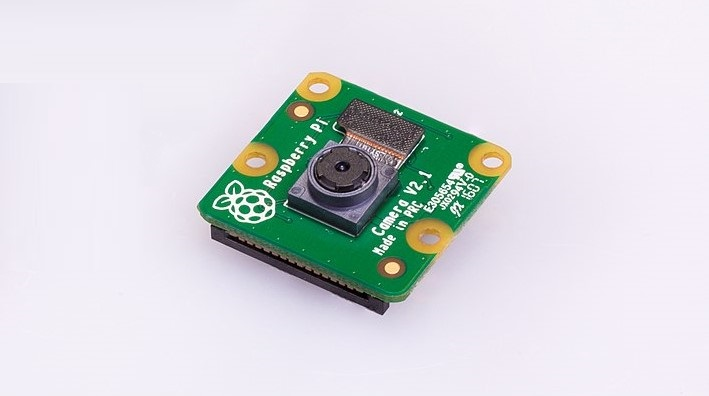
\includegraphics[width=0.6\myImageWidth]{Bilder/piCam.jpg}
	\caption[Raspberry Pi Camera V2.1]{Raspbarry Pi Camera V2.1 (Quelle: \cite{foundationEnglishRaspberryPi2018})}
	\label{fig:PiCAM}
\end{figure}

Die Anzeige der Belegung des Parkhauses soll für Studenten und Mitarbeiter der Hochschule Coburg über ein beliebiges Endgerät aus erreichbar sein.
Aus diesem Grund ist es sinnvoll eine Multi-Plattform Applikation zu erstellen.
Diese sollte auf den gängigsten Betriebssystemen, wie Android, iOS, Windows oder im Web erreichbar sein.
Diese Anwendungen werden häufig durch Frameworks, wie Flutter, Xamarin (mittlerweile .NET MAUI) oder React Native, realisiert.
Die Wahl des verwendeten Frameworks fällt auf Flutter, da dies das aktuell modernste und verbreitetste Framework zur Erstellung nativer Multi-Plattform Anwendungen ist und außerdem bereits Erfahrungen mit dessen Programmierung gemacht wurden.
Die Realisierung mittels einer reinen Web-Anwendung wäre ebenfalls möglich gewesen.
Flutter bietet jedoch die Erstellung von sowohl Web-Anwendungen als auch Applikationen für verschiedene Betriebssysteme.

Als Bindeglied zwischen Raspberry Pi und Applikation für den Nutzer muss ein Server für das Handling der Daten implementiert werden.
Die Schnittstelle zum Server kann über HTTP-Anfragen realisiert werden.
Dieses Konzept ist weit verbreitet und Go, was zur Implementierung des Servers eingesetzt wurde, bietet hierfür hocheffiziente Bibliotheken.
Für die Schnittstelle zur Applikation ist es sinnvoll, eine Methode zu verwenden, welche es dem Server erlaubt, Daten zu schicken, ohne eine Anfrage zu erhalten.
So kann sichergestellt werden, dass die Anzeige der Anwendung stets mit dem Auslastungs-Wert des Servers übereinstimmt und hierfür kein Polling notwendig ist.
Ein dafür häufig verwendetes Protokoll, das auch in dieser Arbeit verwendet wird, ist MQTT.\@

\selectlanguage{ngerman}
\section{Technische Umsetzung}\label{ch:Umsetzung}
Das im Rahmen dieser Arbeit entwickelte System besteht aus drei Teil-Systemen: dem Sensor, dem Server und der App.
Dabei wird unter dem Sensor System der Teil angesehen, welcher eine klassische Detektion ersetzen kann.
Der Server stellt die das Bindeglied der Kommunikation zwischen Sensor und App dar.
Für den Nutzer werden die erfassten Daten in der App dargestellt die vom Server gesendet werden.
Die gesamte Architektur ist in Abbildung~\ref{fig:Architektur} dargestellt.

\begin{figure}[h]
    \myImagePos{}
    \includesvg[inkscapelatex=false,width=\myImageWidth]{Bilder/Architektur_gesamt_2.svg}
    \caption[Schematische Darstellung der System-Architektur]{Schematische Darstellung der System-Architektur mit ihren einzelnen Systemen (blau), den an diesen angebundenen Komponenten (hellblau) und den zur Kommunikation verwendeten Protokollen (grün). (Quelle: eigene Darstellung)}
    \label{fig:Architektur}
\end{figure}

Im Folgenden wird jeweils auf die Umsetzung der einzelnen Teil-Systeme eingegangen.

\selectlanguage{ngerman}
\subsection{Sensor}\label{ch:Umsetzung_Sensor}
% - Objekterkennung auf Frames: vortrainierte Modelle
% - Schwierigkeit: Nicht nur Erkennung einzelner Objekte nötig, sondern Erkennung des Rein- und Rausfahrens der Autos
%     --> zwei Implementierungen, Verweis auf Tests

Die Komponente, welche erkennt, wie viele Autos den Parkplatz befahren und verlassen, wird in dieser Arbeit Sensor genannt, besteht aus einem Mini-Computer und einer Kamera.
Für die konkrete Anwendung (siehe Kapitel~\ref{ch:Test}) wurde ein Raspberry Pi Model B+ und ein Pi Camera Module v2.1 verwendet.
Auf diesem läuft kontinuierlich eine Software, welche den Kamera-Input verarbeitet und hieraus die rein- und rausfahrenden Autos erkennt.
Die Herausforderung besteht darin, nicht nur die Erkennung einzelner Fahrzeuge in den einzelnen Frames zu ermöglichen, sondern auch das Ein- und Ausfahren der Fahrzeuge zu identifizieren.
Um dieses Problem zu lösen, werden zwei verschiedene Implementierungen, welche im Folgenden erklärt werden, entwickelt und in Kapitel~\ref{ch:Test} getestet.

\subsubsection{Variante 0: einfache Objekterkennung}\label{ch:Sensor_v0}
% - sehr performant
% - viel zu ungenau
Zunächst wird versucht, eine Objekterkennung mit dem OpenCV-Framework umzusetzen.
Das Verfahren verwendet Computer-Vision-Techniken wie Hintergrundsubtraktion und Konturen\-erkennung, um Fahrzeuge in einem Video zu erkennen und zu zählen.
Dabei werden Bewegungsunterschiede zwischen Frames erkannt und die Konturen bewegter Objekte identifiziert, um potenzielle Fahrzeuge zu identifizieren.
Die Anzahl der Fahrzeuge wird basierend auf der Position der Konturzentren ermittelt.
Nach den ersten Tests stellt sich das Verfahren allerdings als unbrauchbar heraus.
Das Verfahren ist zwar sehr performant, sodass bis zu 30 Bilder pro Sekunde verarbeitet werden können, die Genauigkeit ist für die Umsetzung des Projektes jedoch zu gering.
Teilweise werden einzelne Fahrzeuge als mehrere gezählt.
Weiterhin gibt es mehrere Objekte und Personen, die von dieser Methode fälschlicherweise als Fahrzeug erkannt werden.
Deshalb wird diese Variante nicht weiter verfolgt und verbessert.

\subsubsection{Variante 1: Richtung des Bewegungsvektors}\label{ch:Sensor_v1}
% - Grundidee: Erkennen in welche Richtung im Bild (oben oder unten) Auto fährt
% - Vorgehen: 
%     - Rechtecke (Eckkoordinaten) der Autos durch Objekterkennung
%     - Berechnung der Mittelpunkte
%     - Berechnung der Bewegungsrichtung 
%         - Für jeden Punkt im aktuellen Frame werden die Distanzen zu den Punkten des vorherigen Frames errechnet
%         - Der Punkt mit der jeweils kürzesten Distanz wird ausgewählt und mit diesem der Bewegungsvektor errechnet. Falls bereits passender früherer Bewegungsvektor vorhanden, wird Aufaddiert, da nur Gesamtergebnis wichtig  
%         - Punkte des vorherigen Frames, die für keinen aktuellen Punkt die kürzeste Verbindung waren (weil jetzt weniger Autos im Bild), werden gesucht und deren Bewegungsvektor für Zählung verwendet 
%     - Anhand der Richtung der y Koordinate es Vektors die Richtung (oben/unten) des Autos bestimmen 
%     - API Aufruf

Um Autos nur einmal zu erkennen wurde ein anderer Ansatz verfolgt, der im Folgenden beschrieben wird.

Die Grundidee des Algorithmus besteht darin, die Richtung zu ermitteln, in die ein Fahrzeug im Bild fährt.
Hierbei wurde die vereinfachte Annahme getroffen, dass Autos, die sich im Kamerabild nach oben bewegen, aus dem Parkhaus fahren, während Autos, die sich nach unten bewegen, in das Parkhaus hinein fahren.
Diese Annahme gilt nur, wenn die Kamera von oben aus dem Inneren des Parkhauses die Ein- und Ausfahrt filmt.
Andernfalls müssten die Richtungen entsprechend angepasst werden.

Zunächst werden die Fahrzeuge in den einzelnen Frames mithilfe von einem vortrainierten Modell, konkret YOLOv5~\cite{yolov5}, für die Objekterkennung identifiziert.
Die Eckkoordinaten der erkannten Fahrzeuge werden dann verwendet, um die Mittelpunkte der Fahrzeuge zu berechnen.
Die Berechnung der Bewegungsrichtung auf Basis der Mittelpunkte erfolgt in mehreren Schritten.
Hierfür werden für jeden Punkt im aktuellen Frame die Distanzen zu den Punkten des vorherigen Frames ermittelt.
Hiervon wird jeweils der Punkt mit der kürzesten Distanz ausgewählt und der Bewegungsvektor zwischen den zwei Punkten berechnet.
Sollte bereits ein passender Bewegungsvektor für den Punkt aus vorherigen Frames vorhanden sein, wird dieser Vektor aufaddiert, da nur das Gesamtergebnis relevant ist.
Der hieraus resultierende Vektor zeigt also von der ersten Sichtung des Autos zu seiner aktuellen Position und ist in Abbildung~\ref{fig:Variante1} blau dargestellt.

\begin{figure}[h]
	\myImagePos{}
	\includegraphics[width=\myImageWidth]{Bilder/Methode2_Beispiel.png}
	\caption[Fahrzeugerkennung Variante 1 Beispiel]{Beispiel der Fahrzeugerkennung mit Variante 1 (Quelle: eigene Darstellung)}
	\label{fig:Variante1}
\end{figure}

Zur Zählung werden die errechneten Bewegungsvektoren verwendet, wenn das entsprechende Auto das Kamerasichtfeld verlassen hat.
Das ist der Fall, wenn Punkte des vorherigen Frames für keinen Punkt im aktuellen Frame die kürzeste Verbindung darstellten, weil jetzt weniger Autos im Bild zu sehen sind als im vorherigen Frame.
In diesem Fall werden die zuvor berechneten Bewegungsvektoren der nicht zugeordneten Punkte für die Zählung verwendet.
Selbst wenn zwischen den Frames ein neues Auto in den Bildausschnitt fährt, während ein anderes ihn verlässt, stellt dies kein Problem dar, weil dies aufgrund eines Schwellwerts nur für Autos passieren kann, die in entgegengesetzte Richtungen fahren und sich die aufaddierten Bewegungsvektoren folglich ausgleichen, sodass der Zählerwert ebenso unverändert bleibt.
In Abbildung~\ref{fig:Variante1} ist in Weiß der Vektor des vorherigen Autos zu sehen.

Die Richtung des Fahrzeugs wird anhand der y-Koordinate des Bewegungsvektors bestimmt.
Wenn die y-Koordinate des Vektors positiv ist, fährt das Fahrzeug nach unten, andernfalls fährt es nach oben, was durch die bereits erwähnte Vereinfachung einen Rückschluss auf die tatsächliche Fahrtrichtung des Autos ermöglicht.
Der interne Zähler des Sensors wird daraufhin entsprechend inkrementiert oder dekrementiert und über eine HTTP PUT-Request im, in Kapitel~\ref{ch:Umsetzung_Server} beschrieben Format, als JSON an den Server übertragen.

\subsubsection{Variante 2: Überschreiten einer Linie}\label{ch:Sensor_v2}
% - Grundidee: Einteilen des Videos in zwei Bereiche (horizontal - z. B. Einfahrt des Parkhaus)- bei Änderung des Bereichs -> hoch- oder runterzählen
% - Vorgehen:
% 	- Mittelpunkt der Objekterkennung
%	- jedes Auto mit ID versehen
%	- schauen in welchem Bereich sich ID befindet
% 	- Bei Änderung des Bereichs hoch bzw. runterzählen
%		- API Aufruf

Die grundlegende Idee des Algorithmus besteht darin, Fahrzeuge in den Frames eines Videos mithilfe von YOLOv8 zu identifizieren und dann ihre Bewegung in Bezug auf eine festgelegte Linie zu verfolgen, um die Fahrtrichtung zu bestimmen.
Die Linie wird dabei horizontal über der Einfahrt des Parkhauses festgelegt, wie dies in Abbildung \ref{fig:Variante2} zu sehen ist.
Somit wird das Bild in zwei Zonen geteilt.
Ändert sich die Position eines Autos von der oberen in die untere Zone des Bildes, so wird die Anzeige der freien Parkplätze um eins verringert, da sich nun ein Auto mehr im Parkhaus befindet.
Geschieht eine Änderung der Position von unten nach oben, so wird die Anzeige um eins erhöht.

\begin{figure}[h]
	\myImagePos{}
	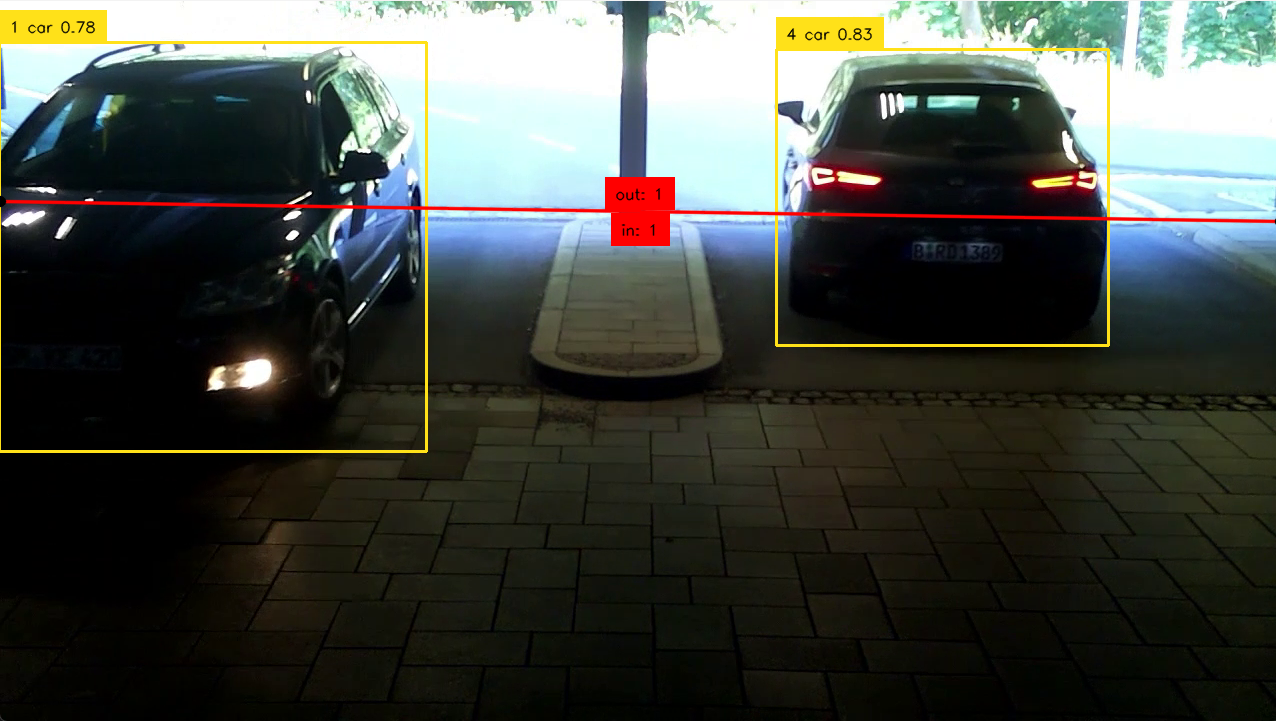
\includegraphics[width=\myImageWidth]{Bilder/Method3_Beispiel.png}
	\caption[Fahrzeugerkennung Variante 2 Beispiel]{Beispiel der Fahrzeugerkennung mit Variante 2 (Quelle: eigene Darstellung)}
	\label{fig:Variante2}
\end{figure}

Es wird YOLOv8 eingesetzt, um die Fahrzeuge in den einzelnen Frames des Videos zu erkennen.
Der Vorteil des Frameworks ist es, dass es Objekten IDs zuordnen kann.
Somit ist eine eindeutige Zuordnung eines Autos über mehrere Frames hinweg möglich.
Die Zuordnung einer ID zu einem konkreten Auto über eine gewisse Dauer geschieht über verschiedene Merkmale des Objektes, wie die Eckpunkte der Objekterkennung, die Geschwindigkeit des Autos oder die Veränderung der Zuverlässigkeitswerte des Algorithmus.
Die erkannten Fahrzeuge werden durch ihre Eckkoordinaten repräsentiert.
Der daraus errechnete Mittelpunkt gibt Aufschluss über die Position des Fahrzeuges.

Der Algorithmus nutzt die erfassten Zählerwerte, um die aktuelle Auslastung des Parkhauses an einen Server zu übertragen.
Dazu wird eine HTTP PUT-Request im JSON-Format verwendet, um die Zählerwerte an den Server zu senden und die Fahrzeugbewegungen zu protokollieren.
\selectlanguage{ngerman}
\subsection{Server}\label{ch:Umsetzung_Server}
% - Geschrieben in Go 
% - Input als HTTP Schnittstelle
%   - in Produktion: Verwendung von HTTPS
%       - dann Basic Auth kein Problem 
%       - jeder Sensor hat Username (site_id) und Passwort das (als Hash) manuell in die SQLite DB eingetragen werden muss
%       - sowieso Pushen, daher egal ob Publish via MQTT oder HTTP Request (PUT)
% - Output als HTTP und MQTT 
%   - Vorteil MQTT: Abonnieren statt Pullen
%   - MQTT: 
%       - Topic ist die site_id
%       - beim Verbinden wird letzter Stand geschickt (retain=true)
%       - Server ist Broker
%       - Clients dürfen nur subscriben, nicht publishen; jeder darf verbinden (keine Beschränkung auf IP-Adressen oder Anmeldung mit Passwort)
% - Anbindung an SQLite DB
%   - 2 Tabellen
%   - sites: Speicherung der Zugangsdaten
%   - counter: Speicherung der Zählerstände
% - ursprünglicher Eintrag (Maximale Anzahl der Autos (max_cars), Anzeigename des Parkplatzes (display_name), ID (site_id) und Passwort Hash (password_hash)) in DB muss manuell geschehen
%   - In finalem Produkt wäre ggf. zusätzliche Anwendung für Mitarbeiter notwendig

Der Server wurde in der Programmiersprache Go entwickelt und dient zur Verwaltung und als zentrale Stelle der Kommunikation für die Übermittlung der Zählerwerte von Sensor zum Endnutzer.

Zum Entgegennehmen der Werte vom Sensor wird die HTTP-Schnittstelle \lstinline|PUT /api/v1/c/{site_id}| zur Verfügung gestellt.
Die Daten werden für diese im HTTP Body in JSON übertragen.
Das vom Server erwartete JSON Objekt, welches nachfolgend beispielhaft dargestellt ist, enthält dabei aktuell lediglich das Attribut \lstinline|currentCars|, welches den aktuellen Zählerstand als Ganzzahl enthält.

\lstset{language=json, numbers=none}
\begin{center}
    \begin{mylisting}[hbox,enhanced,drop shadow]{Input JSON}
{
    "currentCars": 60
}
    \end{mylisting}
\end{center}

Damit diese HTTP-Request zum Ändern des Zählerstandes nicht von jedem ungeschützt verwendet werden kann, ist eine Authentifikation nötig.
Konkret besitzt hierzu jeder Sensor, der mit dem Server verbunden ist, einen eindeutigen Benutzernamen (\lstinline|site_id|) sowie ein Passwort.
Zur Authentifizierung mit dem Server wird hierzu die HTTP Basic Authentication genutzt, bei welcher Nutzername (\lstinline|site_id|) und Passwort im HTTP Header als Base64 String kodiert übertragen werden.
Auf komplexere Authentifizierungsverfahren, wie beispielsweise JSON Web Tokens (JWT) wurde verzichtet, da die gebotenen Vorteile, wie beispielsweise die Möglichkeit zum clientseitigen Ausloggen, das automatische Ablaufen des Tokens oder der Schutz vor Klau des Passworts durch Verwendung des Tokens, in diesem Anwendungsfall als API nicht benötigt werden.
Zu Entwicklungszwecken wurde bisher auf die Verwendung von einer verschlüsselten Datenübertragung mittels HTTPS verzichtet.
In einer Produktivumgebung sollte zwingend \mbox{HTTPS} verwendet werden, um eine geschützte Übertragung zu gewährleisten.
Besonders wichtig ist dies, weil ohne verschlüsselte Verbindung das Passwort abgefangen werden kann.

Als Ausgabeschnittstelle stellt der Server die Daten sowohl über HTTP als auch über MQTT bereit.
Mittels HTTP kann über die Schnittstelle \lstinline|GET /api/v1/c/{site_id}| das JSON Objekt, welches nachfolgend beispielhaft zu sehen ist, mit den Zählerinformationen abgerufen werden.
Der Vorteil von MQTT besteht darin, dass Clients Daten abonnieren können, anstatt sie aktiv abzurufen.
Der Server fungiert als MQTT-Broker und Clients können sich mit ihm verbinden, um Topics zu abonnieren und bei Änderungen dieser die Daten zu empfangen.
Die \lstinline|site_id| wird hierbei als Topic des MQTT-Protokolls verwendet.
Sobald vom Sensor, wie zuvor beschrieben, mittels HTTP der Zählerstand aktualisiert wird, publisht der Server diesen auf die entsprechende MQTT-Topic.
Beim Verbinden mit dem MQTT-Server wird der letzte bekannte Zustand an den Client gesendet, da das \lstinline|retain|-Flag auf \lstinline|true| gesetzt ist.
Somit sind direkt aktuelle Daten verfügbar, ohne dass zunächst eine Änderung durch den Sensor gemeldet werden muss.
Die Clients haben jedoch keine Berechtigung, Daten zu veröffentlichen (publishen).
Es gibt daher keine Beschränkungen für die MQTT-Verbindung aufgrund von IP-Adressen oder Anmeldungen mit Passwörtern.

\lstset{language=json, numbers=none}
\begin{center}
    \begin{mylisting}[hbox,enhanced,drop shadow]{Output JSON}
{
    "id": "HS_Coburg",
    "displayName": "Parkhaus Hochschule Coburg",
    "currentCars": 100,
    "maxCars": 530
}
    \end{mylisting}
\end{center}

Zur Speicherung der relevanten Informationen verwendet der Server eine SQLite-Datenbank mit zwei Tabellen.
Die erste Tabelle, \lstinline|counter|, speichert die aktuellen Zählerstände sowie gleichbleibende Daten der Sensoren, wie beispielsweise die maximale Anzahl der Autos, die im JSON der Ausgabeschnittstelle vorhanden sind.
Die zweite Tabelle, \lstinline|sites|, enthält die Zugangsdaten für die einzelnen Sensoren.
Das Passwort wird hierbei nur als Hash-Wert gespeichert.
Die Einträge zu Zugangsdaten und Details der Parkplätze müssen zuvor manuell in die Datenbank eingetragen werden.
Hierzu wäre es in einem finalen Produkt möglicherweise erforderlich, eine zusätzliche Anwendung für Mitarbeiter bereitzustellen.
Diese Anwendung könnte eine Benutzeroberfläche bieten, um neue Sensoren hinzuzufügen, ihre Zugangsdaten einzugeben und weitere Konfigurationen vorzunehmen.
Für den Rahmen des aktuellen Prototyps genügt die Oberfläche von Drittanbieter Datenbanksoftware, wie beispielsweise der \textit{DB Browser for SQLite}.

\selectlanguage{ngerman}
\subsection{App}\label{ch:Umsetzung_App}
% - Geschrieben mit Flutter und Dart
%   --> verschiedene Plattformen (Android, Windows, iOS, macOS, ...)
% - abonniert via MQTT die Topic (im Prototyp ist Topic hartkodiert; final Auswahl aus Liste, wenn allgemeine App)

Um die aktuelle Parkhausbelegung für den Nutzer darzustellen, wurde eine App entwickelt, die mithilfe von Flutter und Dart geschrieben wurde und daher verschiedene Plattformen, wie Android, Windows, iOS und macOS, bedient.
In Abbildung~\ref{fig:app} sind Screenshots der App dargestellt.

\begin{figure}[h]
	\centering
	\subfloat{
		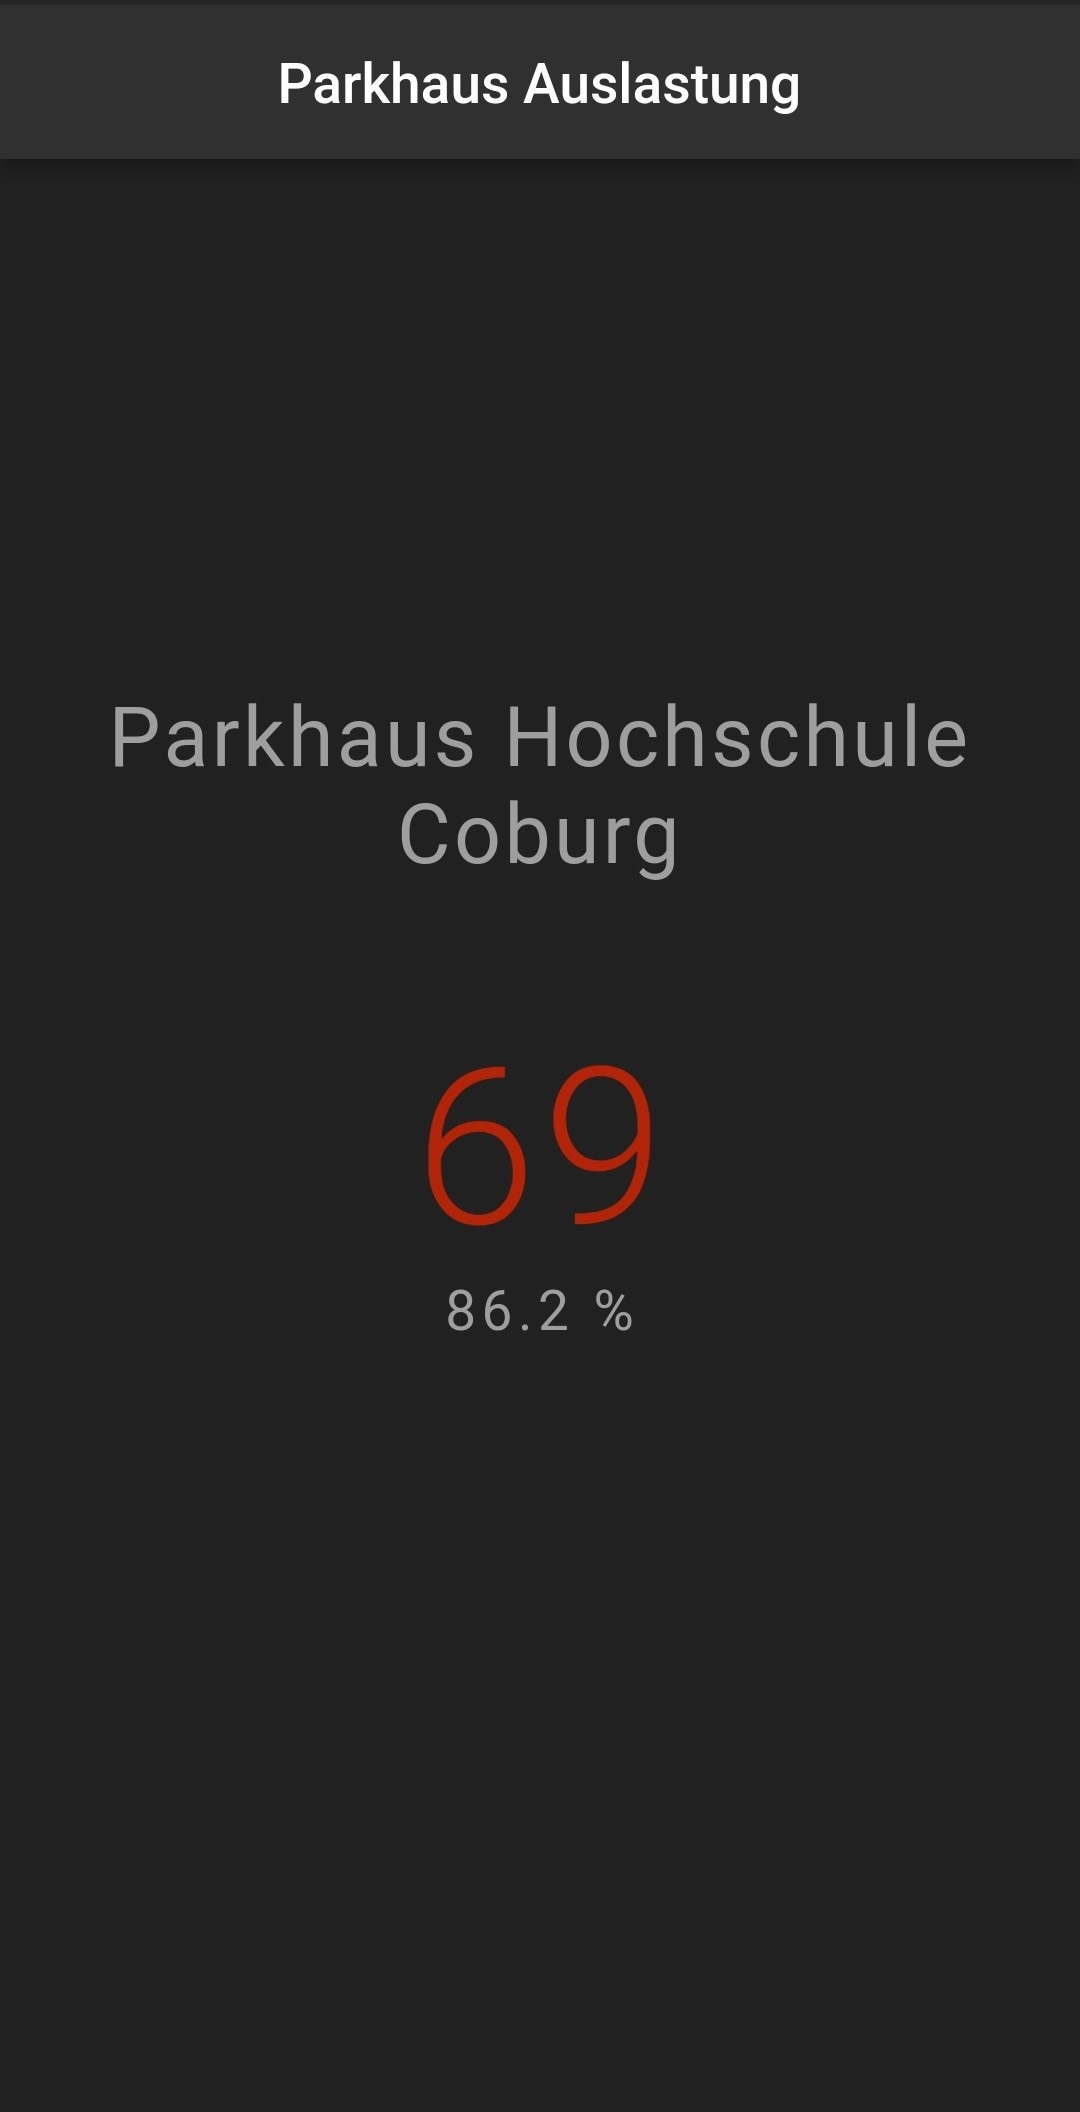
\includegraphics[width=0.3\myImageWidth]{Bilder/app_69.jpg}}
	\hfill
	\subfloat{
		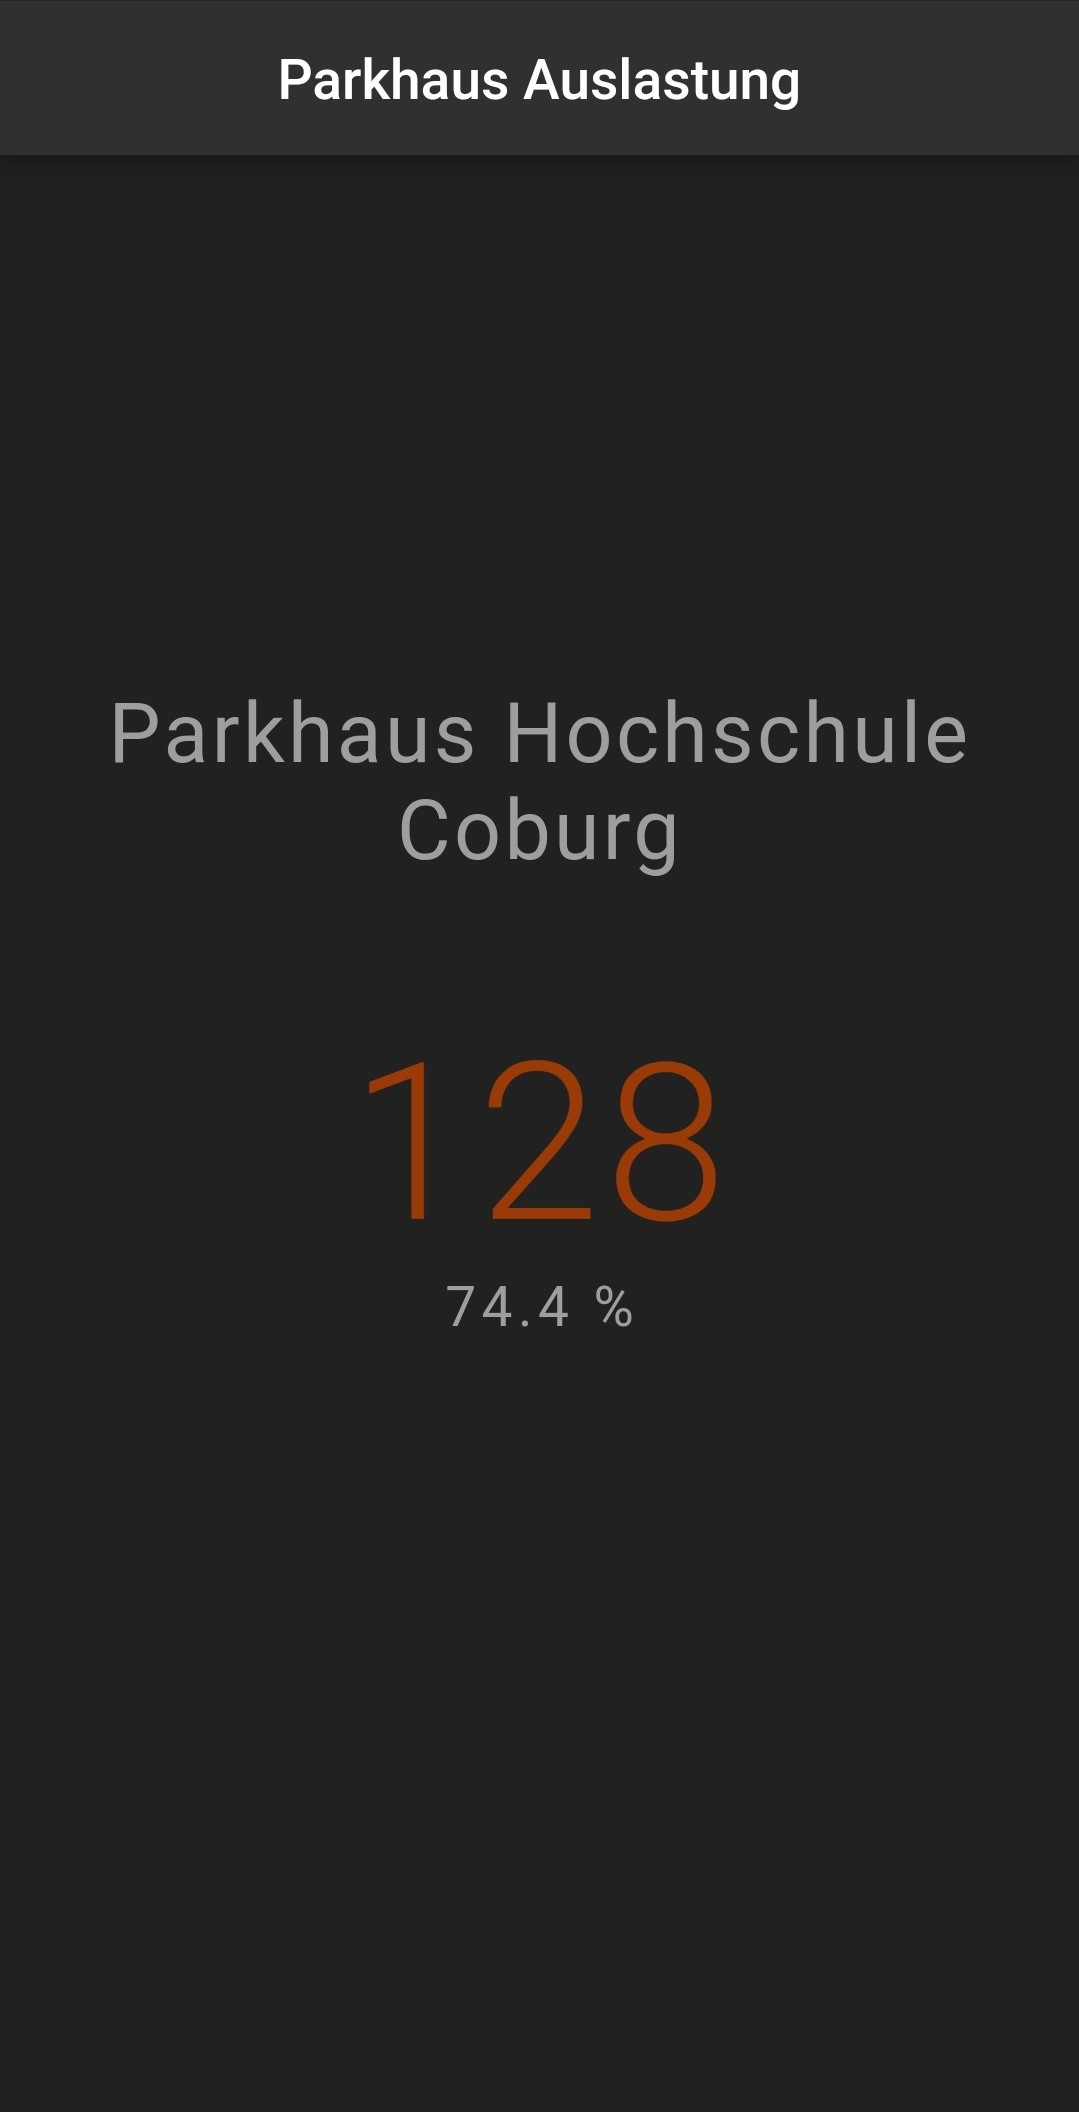
\includegraphics[width=0.3\myImageWidth]{Bilder/app_128.jpg}}
	\hfill
	\subfloat{
		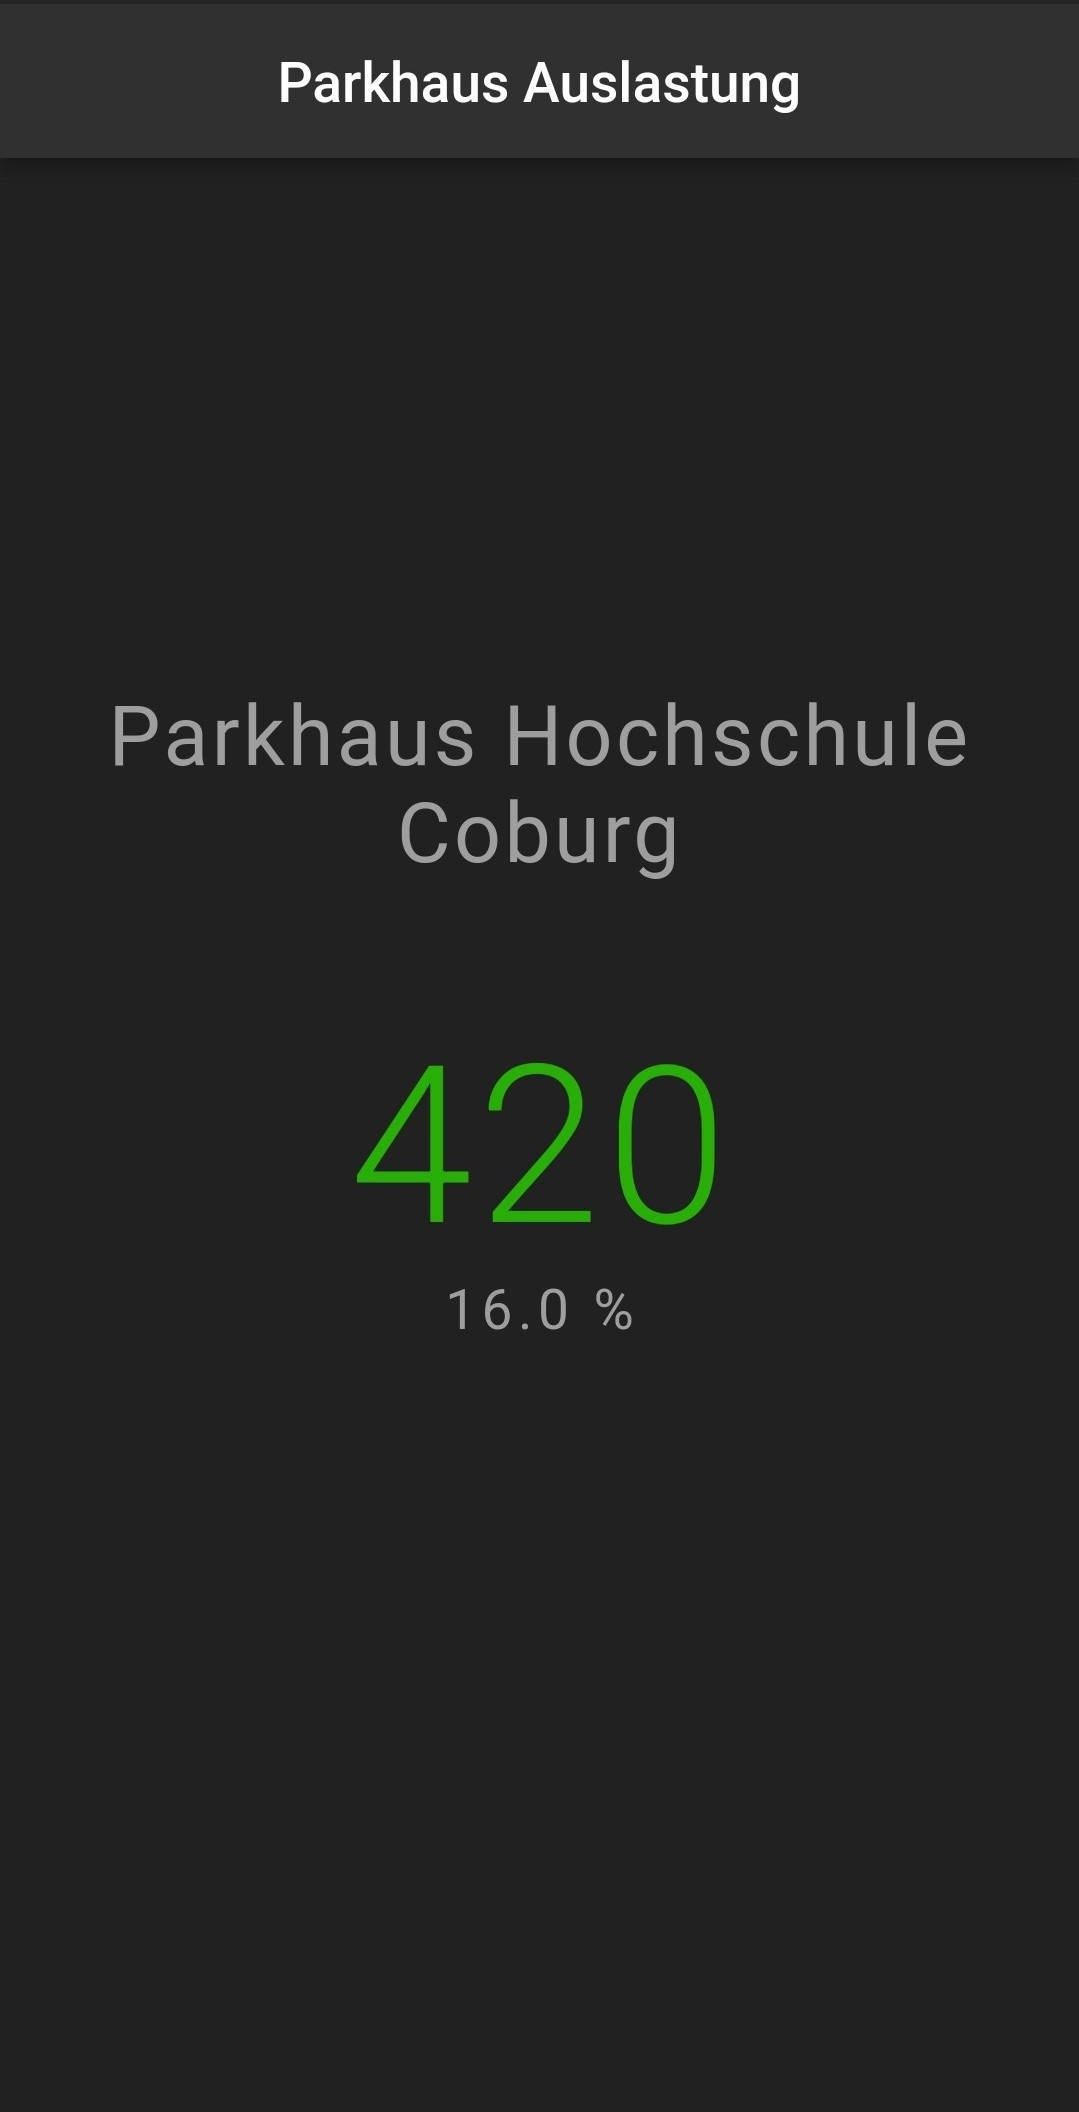
\includegraphics[width=0.3\myImageWidth]{Bilder/app_420.jpg}}
	\caption[Screenshots der App]{Screenshots der App (Quelle: eigene Darstellung)}\label{fig:app}
\end{figure}

Flutter und Dart stellen ein leistungsstarkes Framework und eine Programmiersprache dar, die von Google entwickelt wurden, um die Entwicklung plattformübergreifender Apps zu vereinfachen.
Flutter ermöglicht die Erstellung reaktiver Benutzeroberflächen, während Dart eine effiziente und objektorientierte Programmierung unterstützt.
Die Verwendung einer einzigen Codebasis für verschiedene Plattformen verbessert die Wartung und Skalierbarkeit der App erheblich.~\cite{awsWasIstFlutter}~\cite{dartDartOverview}

Wie bereits genannt, dient MQTT als leichtgewichtiges und zuverlässiges Kommunikationsprotokoll zum Empfangen der Nachrichten.
Die App abonniert die Topic des entsprechenden Parkplatzes beim Broker, um diese Informationen anzuzeigen.
Im aktuellen Prototypen ist die Topic hartkodiert.


\selectlanguage{ngerman}
\section{Anwendung und Test}\label{ch:Test}
% TODO:
% - Installation in Parkhaus und Aufzeichnung
%   - Zu Testzwecken separat von Erkennung
% - Allgemeine Erklärung zur Nutzung des Systems
% - Vergleich der zwei Zählverfahren

\selectlanguage{ngerman}
\section{Fazit}\label{ch:Fazit}
% Zukünftig:
% - HTTPS
% - Anwendung für Datenbank für Mitarbeiter
% - Auswahl der Parkplätze in App; andere Darstellung in App, bei großflächigem Einsatz beispielsweise auf Karte
% - selbes System für die Mitarbeiterparkplätze --> diese vom Zähler abziehen
% - separates Zählsystem für Mitarbeiter anbieten

Die Anwendung und der Test des entwickelten Fahrzeugzählsystems wurden in einem realen Parkhaus durchgeführt, wobei sich das System als zuverlässig in der Zählung der Fahrzeuge erwies.
Der Vergleich der beiden implementierten Zählverfahren ergab, dass beide Verfahren eine hohe Genauigkeit und Robustheit aufweisen, Verfahren 1 jedoch bei ähnlicher Effizienz konstantere Zeiten benötigt.
Die Ergebnisse dieser Tests sind vielversprechend und zeigen das Potenzial des Systems für den praktischen Einsatz in der Parkhausauslastungsmessung auf.

Für eine Weiterentwicklung des Systems wurden folgende Aspekte identifiziert.

Um die Performance des Systems zu erhöhen, sollten Alternativen für den Mini-Computer in Betracht gezogen werden.
Der Raspberry Pi 3 B+ hat sich für diese Aufgabe als nicht leistungsstark genug herausgestellt.
Vertreter der Jetson-Reihe von NVIDIA oder Single-Board-Computer der ASUS Tinker-Board-Reihe bieten beispielsweise eine deutlich höhere Rechenleistung.
Gleichzeitig werden alle anderen Anforderungen für die Objekterekennung und die Kommunikation zum Server von den genannten Boards erfüllt.

Um die Sicherheit und den Datenschutz zu gewährleisten, sollte eine Umstellung auf HTTPS erfolgen.
Dies würde die Übertragung der Daten verschlüsseln und die Vertraulichkeit der Informationen gewährleisten.
Dadurch wird sichergestellt, dass die erfassten Messdaten und vor allem Zugangsdaten vor unbefugtem Zugriff geschützt sind.

Im aktuellen Prototypen müssen Parkhäuser initial manuell in der Datenbank angelegt werden.
Eine für den großflächigen Einsatz nötige Erweiterung wäre die Implementierung eines Systems, über welches Mitarbeiter bequem und fehlerfrei neue Stationen anlegen können.

Eine Weiterentwicklung der Anwendung könnte eine dynamische Parkplatzauswahl in der App sein.
Statt fester Standortzuweisungen könnten die verfügbaren Parkplätze und Parkhäuser in der App angezeigt werden, wobei die Darstellung bei großflächigem Einsatz auf einer Karte erfolgen könnte.
Dies würde den Benutzern ermöglichen, freie Parkplätze leichter zu finden und die Effizienz des Parkplatzmanagements zu steigern.
Außerdem wäre so nicht für jedes Parkhaus eine eigene App nötig.

Die Einbindung der Mitarbeiterparkplätze in das Zählsystem wäre eine sinnvolle Erweiterung.
In der Umsetzung des Prototyps wird nicht beachtet, dass innerhalb des Parkhauses ein separater Bereich für Mitarbeiter der Hochschule existiert.
Durch Anbringung eines zweiten Sensors und Subtrahieren der Zählergebnisse der Mitarbeiterparkplätze von den Gesamtzählergebnissen kann auch eine Differenzierung zwischen den Bereichen vorgenommen werden.

Zusammenfassend eröffnet die entwickelte Fahrzeugzählungsanwendung eine Vielzahl von Möglichkeiten für zukünftige Verbesserungen und Erweiterungen.
Die Kombination dieser Aspekte könnte das Fahrzeugzählsystem zu einem sinnvollen Werkzeug für ein effizientes und intelligentes Parkplatzmanagement machen.
Bereits der Prototyp konnte zeigen, wie ohne den Einsatz spezieller Hardware eine Zählung ermöglicht wird.


\finishHSCdocument
